% Section content template for individual Educative lessons
% This file contains the actual content for a specific section
% Generated from Educative API section content

% Section: System Design: The Typeahead Suggestion System
% Section ID: 4981044919140352
% Section Slug: system-design-the-typeahead-suggestion-system
% Generated: 2025-12-08T15:11:01.408405

\subsection{Introduction}\label{0yLA38dxuu55QkPCL4jhF}
\\
\textbf{Typeahead suggestion}, also referred to as the \textbf{autocomplete system}, is a front-end functionality that provides real-time search query suggestions as users type. It enables users to search for a known and frequently searched query. This feature comes into play when a user types a query in the search box. The typeahead system provides a list of top suggestions to complete a query based on the user's search history, the current context of the search, and trending content across different users and regions. Frequently searched queries always appear at the top of the suggestion list. The typeahead system doesn't search faster. However, it helps the user form a sentence more quickly. The underlying algorithm determines the relevance and ranking of suggested terms.

\begin{figure}[htbp]
 \centering
 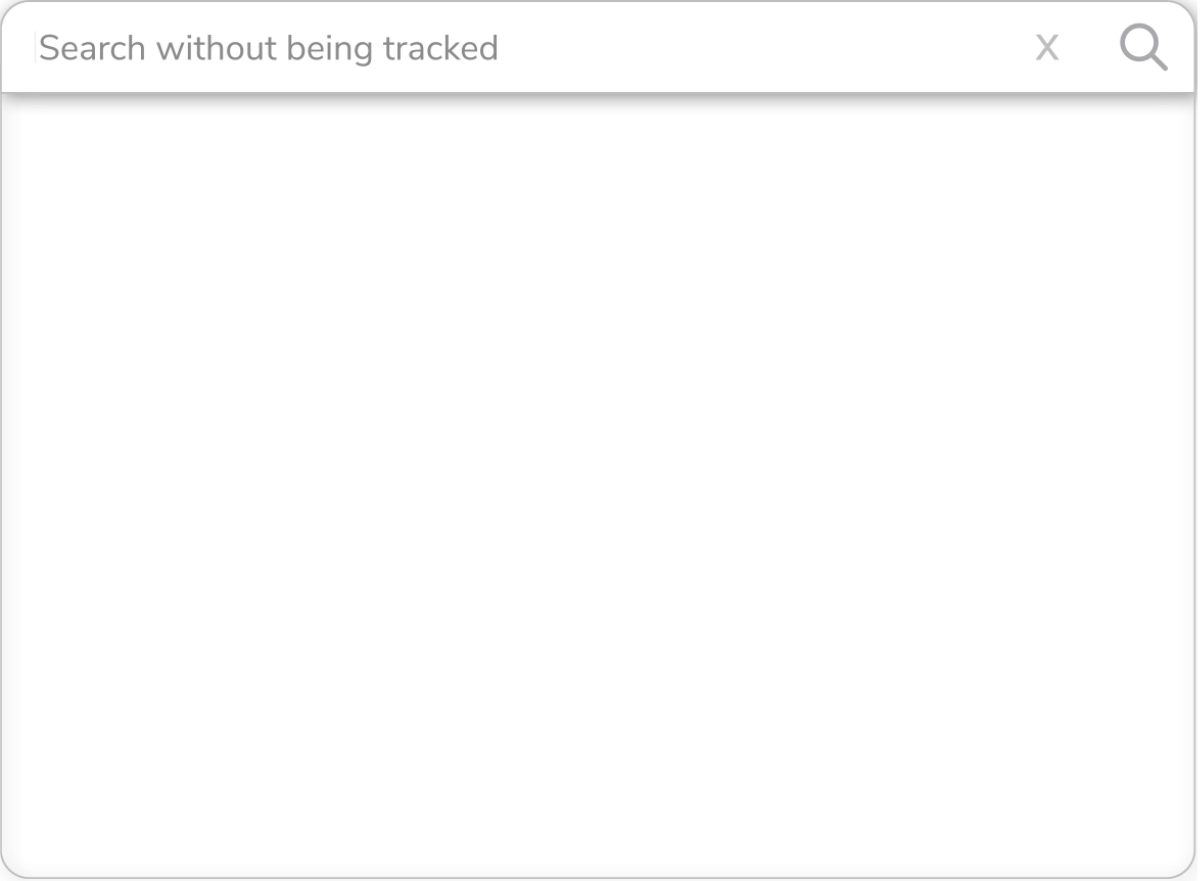
\includegraphics[width=0.25\textwidth]{Images/chapter_37/section_4981044919140352/6394144847429632.png}
 \caption{The typeahead suggestion system in action}
\end{figure}

Typeahead systems are common in applications like:

\begin{itemize}
\item
\protect\phantomsection\label{Jrg1OVJnanVY8-ygCwLX-}
Search engines such as Google or Bing
\item
\protect\phantomsection\label{Ymp-bnf23kEOjOqCk2qT1}
E-commerce websites to autocomplete product names
\item
\protect\phantomsection\label{h8_jdx4T9rZZKrRLgXzke}
Text and code editors
\end{itemize}
\begin{quote}
\textbf{Note:} To deliver a seamless user experience, the system must have low latency and high fault tolerance for typeahead suggestions. The typeahead suggestion systems designed by tech giants, such as Google and Amazon, enhance search accuracy and personalize the user experience by analyzing past interactions and preferences.
\end{quote}
\subsection{Typeahead design problem}\label{dcv2qNCpFVxgsX39mL3mk}
\\
As system designers or a candidate for system design interviews, we should be aware of the workings of the typeahead suggestion system. There could be interesting system design interview questions that an interviewer can ask:

\begin{itemize}
\item
\protect\phantomsection\label{ox1Rgjd5IWY6_2JYF87TU}
How would you design a typeahead suggestion system that is capable of learning from user behavior---how would you incorporate real-time data processing and feedback loops?
\item
\protect\phantomsection\label{yS1zcuIXKCABPVV9NRzoN}
How does load balancer placement and configuration impact the typeahead system performance and user experience?
\item
How would you efficiently update sub-tree structures in a typeahead system to accommodate new data ingestion from various sources, such as web crawlers, etc.?
\end{itemize}

\subsection{A glimpse from the chapter}\label{MiOiJj8z7enwi38-Fca4_}
\\
A robust typeahead system requires careful consideration of several architectural components. For example, key-value stores often support the backend, providing fast data retrieval. Similarly , partitioning the data across multiple application servers enhances scalability and performance. To improve suggestion quality, the offline map-reduce jobs can be used to preprocess and analyze vast amounts of data.
\\
To achieve high availability and fault tolerance of the service, replication of data across servers is necessary. Furthermore , real-time metrics on system performance, such as latency and throughput, are essential for identifying bottlenecks and optimizing the system. Carefully designed interfaces between the frontend and backend, along with effective load balancing, contribute to a seamless user experience across diverse use cases.
\\
Let's move on to the plan to design a typeahead suggestion system.

\subsection{How will we design a typeahead suggestion system?}\label{3ZGdaDuhe92I2ItiXqPF3}
\\
We've divided the chapter on the design of the typeahead suggestion system into six lessons:

\begin{enumerate}
\item
\protect\phantomsection\label{2HZNjGT8tbAG4VcktEZjw}
\href{https://www.educative.io/courses/grokking-the-system-design-interview/requirements-of-the-typeahead-suggestion-systems-design}{\textbf{Requirements}}\textbf{:} In this lesson, we focus on the functional and non-functional requirements for designing a typeahead suggestion system. We also discuss resource estimations for the smooth operation of the system.
\item
\protect\phantomsection\label{WMR-WZuUUPzV6Q_UvWAQq}
\href{https://www.educative.io/courses/grokking-the-system-design-interview/high-level-design-of-the-typeahead-suggestion-system}{\textbf{High-level design}}\textbf{:} In this lesson, we discuss the high-level design of our version of the typeahead suggestion system. We also discuss some essential APIs used in the design.
\item
\protect\phantomsection\label{rLMIL5OH3Ti6EHcfuOISm}
\href{https://www.educative.io/courses/grokking-the-system-design-interview/data-structure-for-storing-prefixes}{\textbf{Data structure for storing prefixes}}\textbf{:} In this lesson, we cover the trie data structure (an efficient tree data structure) that's used to store search prefixes. We also discuss how it can be further optimized to reduce the tree traversal time.
\item
\protect\phantomsection\label{CC7qWTVzp2MI-Xj6B-wY4}
\href{https://www.educative.io/courses/grokking-the-system-design-interview/detailed-design-of-the-typeahead-suggestion-system}{\textbf{Detailed design}}\textbf{:} In this lesson, we explain the two main components, the \emph{suggestions} service and the \emph{assembler}, which make up the detailed design of the typeahead suggestion system.
\item
\protect\phantomsection\label{VVdXoVbvltq6WxezZ9hB7}
\href{https://www.educative.io/courses/grokking-the-system-design-interview/evaluation-of-the-typeahead-suggestion-systems-design}{\textbf{Evaluation}}\textbf{:} This lesson evaluates the proposed design of the typeahead suggestion system based on the non-functional requirements of the system. It also presents some client-side optimization and personalization that could significantly affect the system's design.
\item
\protect\phantomsection\label{t3NPcKnOZfFqo9JWoxmf-}
\href{https://www.educative.io/courses/grokking-the-system-design-interview/quiz-on-the-typeahead-suggestion-systems-design}{\textbf{Quiz}}\textbf{:} In this lesson, we assess your understanding of the design via a quiz.
\end{enumerate}
\\
If you want to gain hands-on experience with building a basic typeahead suggestion system in AWS, consider exploring the following AWS Cloud Lab.

Let's start by identifying the requirements for designing a typeahead suggestion system.

% End of section content